\documentclass[tikz, border=10pt]{standalone}
\usepackage{tikz}
\usepackage{amsmath}
\usepackage{xcolor}

% Define a variable for node distance
 

\begin{document}
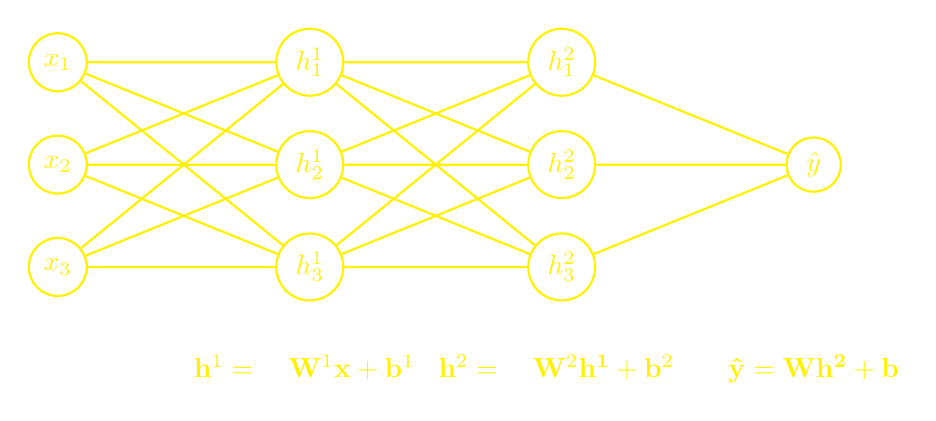
\begin{tikzpicture}[shorten >=0pt, draw=yellow, thick, every node/.style={text=yellow}, xscale=.8, yscale=1.3 ] 
    \tikzstyle{neuron}=[circle, minimum size=12pt, draw=yellow, thick, fill=none]  % Circles with yellow boundary
    \tikzstyle{input neuron}=[neuron];
    \tikzstyle{hidden neuron}=[neuron];
    \tikzstyle{output neuron}=[neuron];
    \tikzstyle{annot} = [text width=4em, text centered]

    % Input layer
    \foreach \x in {1,2,3}
        \node[input neuron] (I-\x) at (0,-\x ) {$x_\x$};

    % Hidden layer 1
    \foreach \x in {1,2,3}
        \node[hidden neuron] (H1-\x) at (4,-\x ) {$h^1_\x$};  
    
    % Hidden layer 1 equation
    \node at (4, -4)  (Hidden1Eq) {
        $\mathbf{h}^1 = \textcolor{white}{f(}\mathbf{W}^1 \mathbf{x} + \mathbf{b}^1\textcolor{white}{)}$
    };

     % Hidden layer 2
     \foreach \x in {1,2,3}
     \node[hidden neuron] (H2-\x) at (8,-\x) {$h^2_\x$};  

    % Hidden layer 2 equation
    \node at (8, -4)  (Hidden2Eq) {
        $\mathbf{h}^2 = \textcolor{white}{f(}\mathbf{W}^2 \mathbf{h^1} + \mathbf{b}^2\textcolor{white}{)}$
    };

    % Output layer
    \node[output neuron] (O) at (12,-2) {$\hat y$};  

    % Output layer  equation
    \node at (12, -4 )  (OutputEq) {
        $\mathbf{\hat y} = \mathbf{W} \mathbf{h^2} + \mathbf{b}$
    };

    % Connect input layer to hidden layer 1
    \foreach \source in {1,2,3}
        \foreach \dest in {1,2,3}
            \draw (I-\source) -- (H1-\dest);

    % Connect input layer to hidden layer 1
    \foreach \source in {1,2,3}
        \foreach \dest in {1,2,3}
            \draw (H1-\source) -- (H2-\dest);

    % Connect hidden layer to output layer
    \foreach \source in {1,2,3}
        \draw (H2-\source) -- (O);
\end{tikzpicture}
\end{document}

